% Beyond the Rate: Oral Presentation (v9)
% Academic Conference — Beamer
\documentclass[aspectratio=169, 11pt]{beamer}

% ── Theme ──
\usetheme{Madrid}
\usecolortheme{whale}
\usefonttheme{professionalfonts}
\setbeamertemplate{navigation symbols}{}
\setbeamertemplate{footline}{%
  \leavevmode\hbox{%
    \begin{beamercolorbox}[wd=.33\paperwidth,ht=2.5ex,dp=1ex,center]{author in head/foot}%
      \usebeamerfont{author in head/foot}\insertshortauthor
    \end{beamercolorbox}%
    \begin{beamercolorbox}[wd=.34\paperwidth,ht=2.5ex,dp=1ex,center]{title in head/foot}%
      \usebeamerfont{title in head/foot}\insertshorttitle
    \end{beamercolorbox}%
    \begin{beamercolorbox}[wd=.33\paperwidth,ht=2.5ex,dp=1ex,right]{date in head/foot}%
      \usebeamerfont{date in head/foot}\insertframenumber{}/\inserttotalframenumber\hspace*{2ex}
    \end{beamercolorbox}}%
  \vskip0pt%
}

% ── Packages ──
\usepackage{amsmath,amssymb}
\usepackage{graphicx}
\usepackage{booktabs}
\usepackage{tikz}
\usetikzlibrary{arrows.meta, positioning, calc}
\usepackage{hyperref}
\usepackage{appendixnumberbeamer}

% ── Colors ──
\definecolor{accent}{RGB}{43, 94, 167}
\definecolor{alertc}{RGB}{192, 57, 43}
\definecolor{success}{RGB}{39, 174, 96}
\definecolor{dimgray}{RGB}{120, 120, 120}

% ── Meta ──
\title[Beyond the Rate]{Beyond the Rate:\\Information Content of FOMC Statement Language}
\author[Yu \& Zhang]{Dechang Yu\inst{1} \and Eileen Zhang\inst{2}}
\institute[XJTLU]{\inst{1} Academy of AI, Xi'an Jiaotong-Liverpool University \and \inst{2} [Affiliation TBC]}
\date{Academic Conference 2026}

\begin{document}

% ═══════════════════════════════════════════════════════════════
% TITLE
% ═══════════════════════════════════════════════════════════════
\begin{frame}[plain]
\titlepage
\end{frame}

% ═══════════════════════════════════════════════════════════════
% OUTLINE
% ═══════════════════════════════════════════════════════════════
\begin{frame}{Outline}
\tableofcontents
\end{frame}

% ═══════════════════════════════════════════════════════════════
\section{Motivation}
% ═══════════════════════════════════════════════════════════════

\begin{frame}{The Puzzle}
\begin{columns}[T]
\column{0.55\textwidth}
\textbf{Central question:}\\
Does FOMC statement language convey information \alert{beyond} the rate decision?

\vspace{1em}
\textbf{Why it matters:}
\begin{itemize}
  \item Central banks increasingly rely on \textbf{forward guidance} as a policy tool
  \item Markets respond to \emph{what the Fed says}, not just \emph{what it does}
  \item The ``information channel'' (Romer \& Romer, 2000) suggests FOMC statements reveal the Fed's superior economic assessment
\end{itemize}

\column{0.42\textwidth}
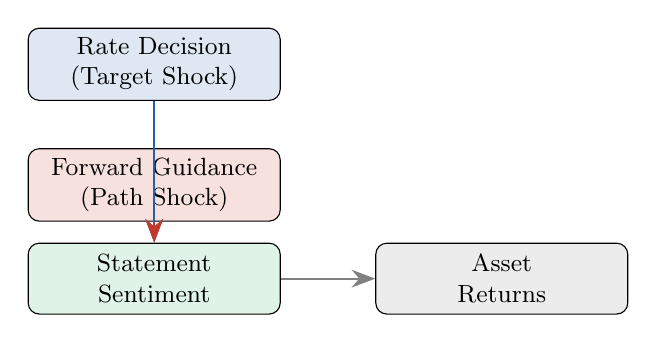
\begin{tikzpicture}[
  box/.style={draw, rounded corners, minimum width=3.2cm, minimum height=0.9cm, align=center, font=\small},
  arr/.style={-{Stealth[length=3mm]}, thick}
]
\node[box, fill=accent!15] (rate) {Rate Decision\\(Target Shock)};
\node[box, fill=alertc!15, below=0.6cm of rate] (fg) {Forward Guidance\\(Path Shock)};
\node[box, fill=success!15, below=1.8cm of rate] (sent) {Statement\\Sentiment};
\node[box, fill=gray!15, right=1.2cm of sent] (asset) {Asset\\Returns};
\draw[arr, accent] (rate) -- (sent);
\draw[arr, alertc] (fg) -- (sent);
\draw[arr, gray] (sent) -- (asset);
\end{tikzpicture}
\end{columns}
\end{frame}

% ═══════════════════════════════════════════════════════════════
\section{Literature \& Contribution}
% ═══════════════════════════════════════════════════════════════

\begin{frame}{Literature}
\begin{itemize}
  \item \textbf{Kuttner (2001)}: 30-min FF futures window $\rightarrow$ isolate monetary policy surprises
  \item \textbf{GSS (2005a)}: Decompose surprises into \textcolor{accent}{target} + \textcolor{alertc}{path} factors
  \item \textbf{Nakamura \& Steinsson (2018)}: High-frequency identification of monetary non-neutrality
  \item \textbf{Campbell et al.\ (2012)}: Delphic vs.\ Odyssean forward guidance
  \item \textbf{Jaroci\'{n}ski \& Karadi (2020)}: Separate policy shock from information shock
  \item \textbf{Hansen et al.\ (2018)}: Computational linguistics for FOMC transparency
  \item \textcolor{success}{\textbf{New (2024--25):}} Chen et al.\ (2025) GPT-4 topic decomposition; Gambacorta et al.\ (2024) CB-LMs; Yao \& Chai (2025) uncertainty-aware LLM
\end{itemize}

\vspace{0.5em}
\textbf{Our contribution:}
\begin{enumerate}
  \item First to directly link \textbf{GSS target/path shocks} to \textbf{FOMC statement sentiment}
  \item Expanded CB dictionary (591 hawkish + 222 dovish terms, fully disjoint)
  \item Formal test of the \textbf{information channel} via text analysis
  \item \textcolor{success}{New:} Dual-equation test, forward-lookingness decomposition, novelty weighting
\end{enumerate}
\end{frame}

% ═══════════════════════════════════════════════════════════════
\section{Data \& Methodology}
% ═══════════════════════════════════════════════════════════════

\begin{frame}{Data}
\begin{columns}[T]
\column{0.48\textwidth}
\textbf{Monetary Policy Shocks}
\begin{itemize}
  \item Acosta (2022): 220 FOMC meetings, 1995--2022
  \item \textcolor{accent}{Target shock}: surprise in current FF rate
  \item \textcolor{alertc}{Path shock}: surprise in future rate path
  \item Extension: USMPD (SF Fed) $\rightarrow$ 2026
\end{itemize}

\vspace{0.5em}
\textbf{Market Data}
\begin{itemize}
  \item CRSP VW/EW/S\&P 500 via WRDS
  \item 117 meetings with complete overlap
\end{itemize}

\column{0.48\textwidth}
\textbf{FOMC Statement Sentiment}
\begin{itemize}
  \item 164 statements, 2006--2025
  \item Expanded CB dictionary:
    \begin{itemize}
      \item 591 hawkish terms
      \item 222 dovish terms
      \item Fully disjoint
    \end{itemize}
  \item Score $= \frac{H - D}{H + D + \epsilon}$
  \item Validated: $r = 0.29$ with rate change
  \item \textcolor{success}{New:} CB-only outperforms combined (R$^2$: 3.90\% vs 1.57\%)
\end{itemize}
\end{columns}
\end{frame}

\begin{frame}{Empirical Strategy}
\textbf{Four hypotheses:}

\vspace{0.5em}
\begin{tabular}{lll}
\toprule
Hypothesis & Prediction & Specification \\
\midrule
H1 & Shocks predict sentiment & $S_t = \alpha + \beta_1 \text{Target}_t + \beta_2 \text{Path}_t + \varepsilon_t$ \\
H2 & Shocks predict returns & $R_t = \alpha + \beta_1 \text{Target}_t + \beta_2 \text{Path}_t + \varepsilon_t$ \\
H3 & Path $>$ Target for sentiment & $|\beta_2| > |\beta_1|$ in H1 \\
H4 & Stronger during FG period & Interaction with FG dummy \\
\bottomrule
\end{tabular}

\vspace{0.8em}
\textbf{Estimation:} OLS with Newey-West (lag=4, data-driven) standard errors

\vspace{0.3em}
\textbf{Sample:} 117 FOMC meetings, January 2006 -- July 2022

\vspace{0.5em}
\textcolor{success}{\textbf{New experiments:}}
\begin{enumerate}
  \item Dual-equation regression (equity + risk premium channels)
  \item Forward-lookingness decomposition (FL vs.\ CA sentiment)
  \item Statement novelty weighting (WLS)
\end{enumerate}
\end{frame}

% ═══════════════════════════════════════════════════════════════
\section{Main Results}
% ═══════════════════════════════════════════════════════════════

\begin{frame}{H1: Sentiment and Monetary Policy Shocks}
\begin{columns}[T]
\column{0.55\textwidth}
\begin{tabular}{lcc}
\toprule
 & Coefficient & $p$-value \\
\midrule
Target shock & 0.000577 & 0.017\textsuperscript{**} \\
Path shock & 0.000633 & 0.152 \\
\midrule
$R^2$ & \multicolumn{2}{c}{1.57\%} \\
$N$ & \multicolumn{2}{c}{117} \\
\bottomrule
\end{tabular}

\vspace{0.5em}
\small
\textsuperscript{***}$p<0.01$, \textsuperscript{**}$p<0.05$, \textsuperscript{*}$p<0.10$

\vspace{0.5em}
\textbf{Key finding:} Target shock is significant at 5\%, path is \alert{not}.\\
Wald test: $\chi^2 = 0.02$, $p = 0.90$ --- cannot reject $\beta_1 = \beta_2$.

\column{0.42\textwidth}
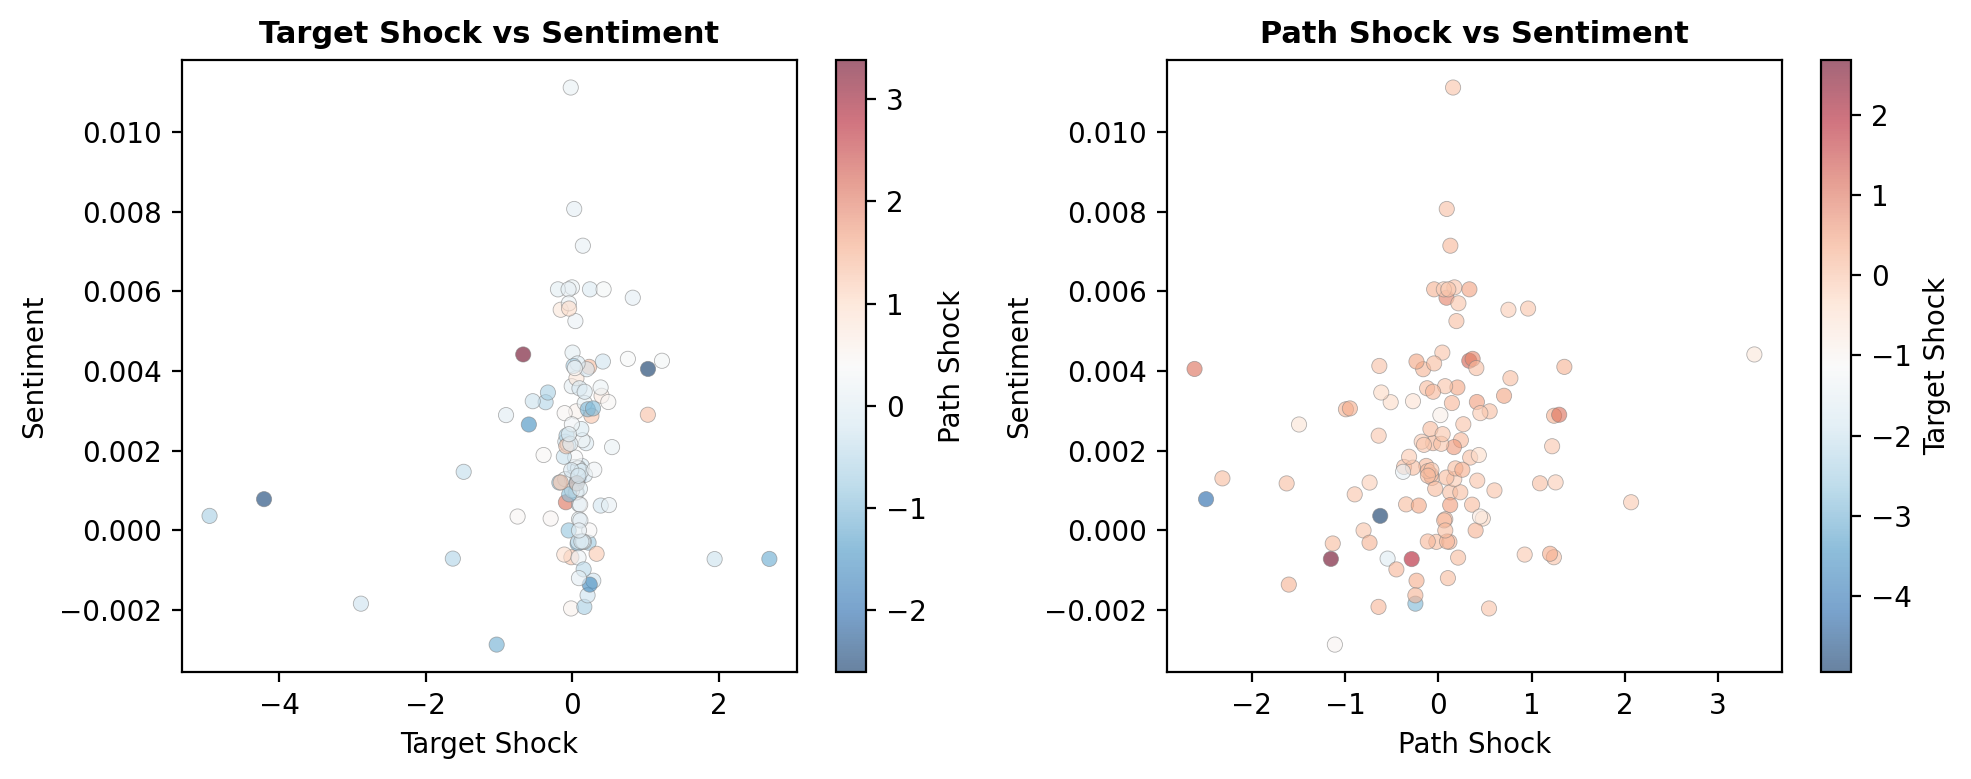
\includegraphics[width=\textwidth]{figures/fig2_scatter.png}
\end{columns}
\end{frame}

\begin{frame}{Sentiment Measure Comparison}
\begin{tabular}{lccc}
\toprule
Measure & $R^2$ & $p$(Target) & $p$(Path) \\
\midrule
CB-only & \textbf{3.90\%} & $<$0.05\textsuperscript{**} & 0.031\textsuperscript{**} \\
Combined (0.5$\times$LM + 0.5$\times$CB) & 1.57\% & 0.017\textsuperscript{**} & 0.152 \\
LM-only & 0.33\% & 0.474 & 0.552 \\
\bottomrule
\end{tabular}

\vspace{0.8em}
\textbf{Key insight:}
\begin{itemize}
  \item CB-only \textbf{doubles} R$^2$ and makes path shock significant at 5\%
  \item LM component adds \alert{noise without signal} for FOMC text (always positive)
  \item Domain-specific dictionaries outperform general-purpose financial dictionaries
\end{itemize}
\end{frame}

\begin{frame}{H2: Asset Returns and Shocks}
\begin{columns}[T]
\column{0.55\textwidth}
\begin{tabular}{lcccc}
\toprule
Asset & $\beta_T$ & $p_T$ & $\beta_P$ & $p_P$ \\
\midrule
CRSP VW & $-0.435$ & 0.043\textsuperscript{**} & $-0.186$ & 0.434 \\
CRSP EW & $-0.449$ & 0.013\textsuperscript{**} & $-0.174$ & 0.421 \\
S\&P 500 & $-0.391$ & 0.073\textsuperscript{*} & $-0.179$ & 0.426 \\
Gold & $-0.404$ & 0.016\textsuperscript{**} & $0.021$ & 0.935 \\
\midrule
\multicolumn{5}{l}{Returns in percentage points; $N = 117$} \\
\bottomrule
\end{tabular}

\vspace{0.5em}
\textbf{Findings:}
\begin{itemize}
  \item Target shock: significant for EW \& Gold
  \item Path shock: \alert{not significant} for any asset
  \item Small-cap sensitivity consistent with literature
\end{itemize}

\column{0.42\textwidth}
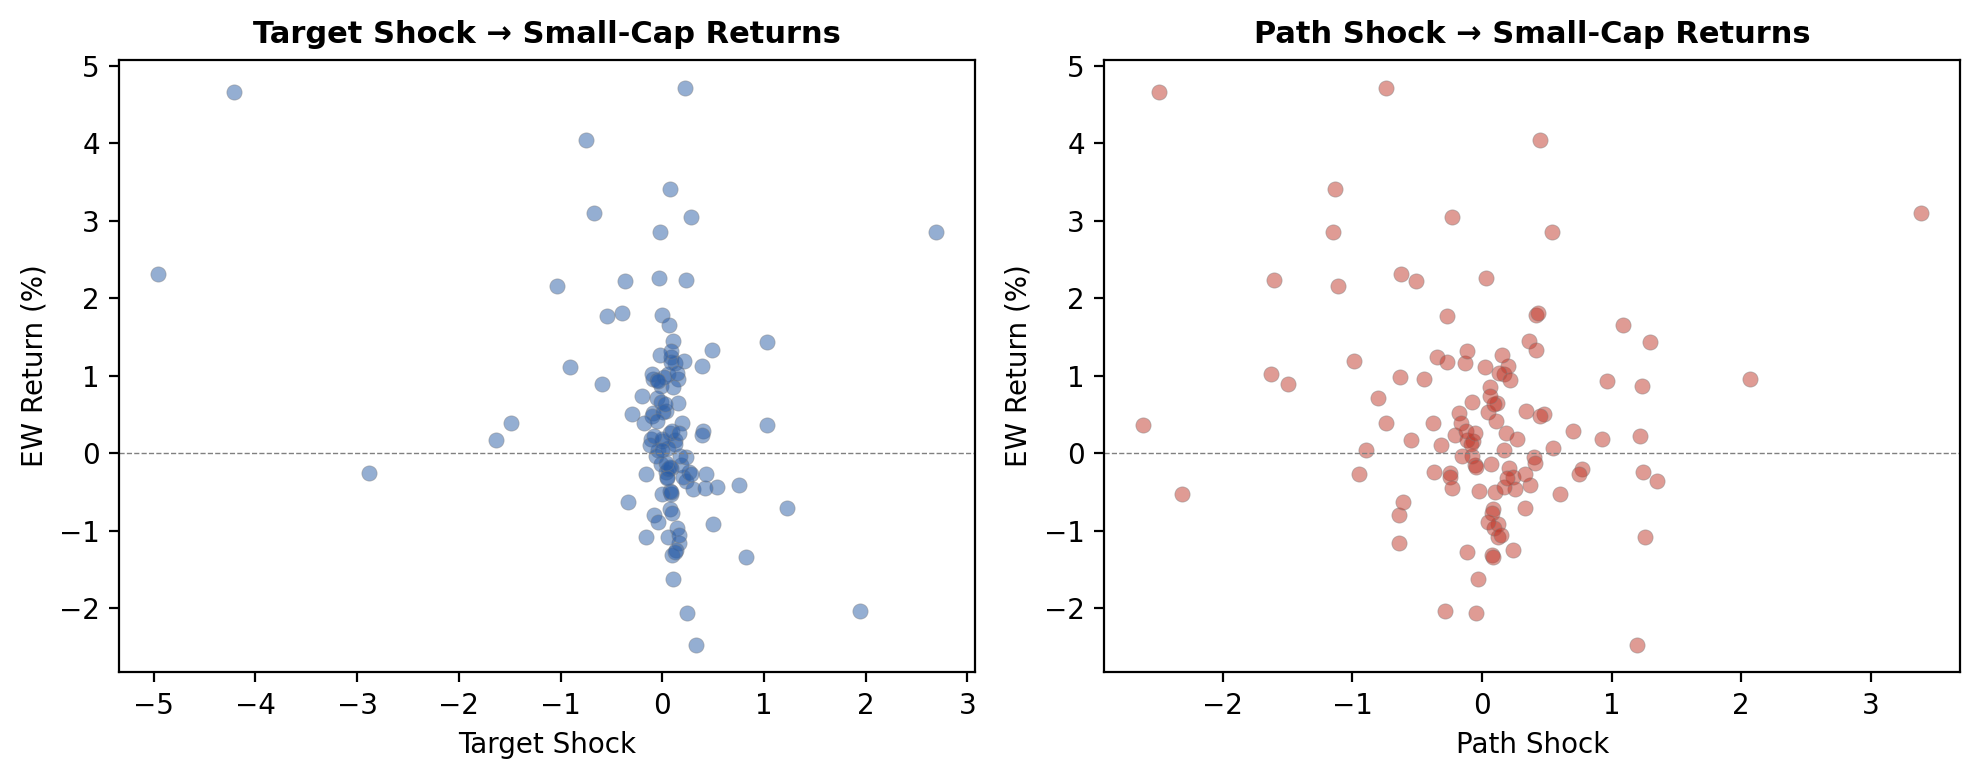
\includegraphics[width=\textwidth]{figures/fig3_h2.png}
\end{columns}
\end{frame}

\begin{frame}{H3 \& H4: Information Channel and Forward Guidance}
\textbf{H3 --- Path $>$ Target?}
\begin{itemize}
  \item Target significant at 5\%, path is not
  \item Wald test: $p = 0.90$ --- cannot reject equality
  \item Evidence is \textit{suggestive}, not definitive
\end{itemize}

\vspace{0.8em}
\textbf{H4 --- Stronger during FG period?}
\begin{itemize}
  \item Sentiment $\times$ FG interaction: $p = 0.602$ (CRSP VW), $p = 0.041$ (NASDAQ, but economically implausible)
  \item \alert{Not robustly significant} --- language channel does NOT strengthen at ZLB
  \item Three interpretations:
    \begin{enumerate}
      \item Shocks absorb information regardless of regime
      \item Dictionary cannot distinguish FG language (cf.\ GPT-3.5 fails 135/139 statements)
      \item FG operates through risk premium channel (Chen et al.\ 2025)
    \end{enumerate}
\end{itemize}
\end{frame}

% ═══════════════════════════════════════════════════════════════
\section{New Experiments}
% ═══════════════════════════════════════════════════════════════

\begin{frame}{Experiment 1: Dual-Equation Regression}
\textbf{Hypothesis:} Forward guidance operates through a risk premium channel (Chen et al.\ 2025)

\vspace{0.5em}
\begin{tabular}{lccc}
\toprule
Dependent Variable & $R^2$ & $p$(Target) & $p$(Path) \\
\midrule
\multicolumn{4}{l}{\textit{Channel 1: Equity Returns (Expectations)}} \\
\quad CRSP VW & 9.1\% & 0.040\textsuperscript{**} & 0.440 \\
\quad S\&P 500 & 7.8\% & 0.072\textsuperscript{*} & 0.426 \\
\midrule
\multicolumn{4}{l}{\textit{Channel 2: Risk Premium (Bond Market)}} \\
\quad 10Y Treasury chg & 0.72\% & 0.403 & 0.890 \\
\quad VIX change & 0.24\% & 0.970 & 0.401 \\
\quad Term spread chg & 1.39\% & 0.667 & 0.341 \\
\bottomrule
\end{tabular}

\vspace{0.5em}
\textbf{Result:} Risk premium channel \alert{not detectable} at daily frequency.\\
\textcolor{dimgray}{\small Consistent with Chen et al.\ using 30-min windows --- channel too fast for daily data.}
\end{frame}

\begin{frame}{Experiment 2: Forward-Lookingness Decomposition}
\textbf{Hypothesis:} Path shock captures forward-looking language (dimension mismatch)

\vspace{0.5em}
\begin{tabular}{lccc}
\toprule
Sentiment Measure & $R^2$ & $p$(Target) & $p$(Path) \\
\midrule
Combined (baseline) & 4.12\% & 0.099 & \textbf{0.015}\textsuperscript{**} \\
Forward-looking only & 0.79\% & 0.012\textsuperscript{**} & 0.800 \\
Current-assessment only & 1.30\% & 0.012\textsuperscript{**} & 0.506 \\
\bottomrule
\end{tabular}

\vspace{0.8em}
\textbf{Counterintuitive finding:}
\begin{itemize}
  \item Path shock is \alert{most significant} in the combined measure ($p = 0.015$)
  \item Path shock is \alert{least significant} in forward-looking sentiment ($p = 0.80$)
  \item \textbf{Dimension mismatch hypothesis rejected}
  \item Path shock captures \textit{broad policy stance signal}, not specifically forward guidance
  \item GSS target/path decomposition $\neq$ FOMC text FL/CA dimensions
\end{itemize}
\end{frame}

\begin{frame}{Experiment 3: Statement Novelty Weighting}
\textbf{Idea:} Not all FOMC statements are equally informative

\vspace{0.5em}
\begin{tabular}{lcc}
\toprule
Method & $R^2$ & Improvement \\
\midrule
Unweighted OLS & 3.98\% & baseline \\
Novelty-weighted WLS & \textbf{5.75\%} & +45\% \\
\bottomrule
\end{tabular}

\vspace{0.5em}
Novelty = cosine distance between TF-IDF vectors of consecutive statements

\vspace{0.8em}
\textbf{Subsample analysis:}
\begin{itemize}
  \item High novelty statements: R$^2$ = 5.78\%
  \item Low novelty statements: R$^2$ = 6.53\%
  \item Difference is small --- novelty helps via weighting, not selection
\end{itemize}

\vspace{0.5em}
\textcolor{dimgray}{\small Absolute R$^2$ remains modest --- measurement innovation alone cannot compensate for daily-frequency limitation.}
\end{frame}

% ═══════════════════════════════════════════════════════════════
\section{Robustness}
% ═══════════════════════════════════════════════════════════════

\begin{frame}{Robustness Checks}
\begin{tabular}{lccccc}
\toprule
Specification & $R^2$ & $p$(Target) & $p$(Path) & $N$ & Period \\
\midrule
Full (Acosta) & 1.57\% & 0.017\textsuperscript{**} & 0.152 & 117 & 2006--22 \\
CB-only & 3.90\% & $<$0.05\textsuperscript{**} & 0.031\textsuperscript{**} & 117 & 2006--22 \\
No COVID & 1.57\% & 0.017\textsuperscript{**} & 0.154 & 115 & 2006--22 \\
Post-2010 & 0.59\% & 0.117 & 0.258 & 97 & 2010--22 \\
Rate change proxy & 0.40\% & 0.323 & 0.323 & 117 & 2006--22 \\
Extended (USMPD) & 1.65\% & 0.419 & 0.058\textsuperscript{*} & 163 & 2006--26 \\
\bottomrule
\end{tabular}

\vspace{0.8em}
\textbf{Key takeaways:}
\begin{itemize}
  \item CB-only sentiment: best specification (R$^2$ = 3.90\%, both shocks significant)
  \item Rate change proxy: 4$\times$ lower R$^2$ --- identification matters
  \item Extended sample: path shock significant at 10\% through 2026
\end{itemize}
\end{frame}

% ═══════════════════════════════════════════════════════════════
\section{Discussion}
% ═══════════════════════════════════════════════════════════════

\begin{frame}{What the New Literature Tells Us}
\begin{columns}[T]
\column{0.48\textwidth}
\textbf{Chen et al.\ (2025): GPT-4 Topics}
\begin{itemize}
  \item Forward guidance operates through \textcolor{alertc}{risk premium channel}
  \item GPT-3.5 fails to identify FG in 135/139 statements
  \item Our CB dictionary has the same limitation
\end{itemize}

\vspace{0.5em}
\textbf{Gambacorta et al.\ (2024): CB-LMs}
\begin{itemize}
  \item Open-weight, domain-specific models
  \item Outperform dictionaries on stance classification
  \item \textcolor{success}{Most promising upgrade path}
\end{itemize}

\column{0.48\textwidth}
\textbf{IMF (2025): Four Dimensions}
\begin{itemize}
  \item Topic + Stance + Sentiment + Forward-lookingness
  \item Topic-level sentiment $>$ aggregate
  \item Our null H4 may reflect aggregation
\end{itemize}

\vspace{0.5em}
\textbf{Yao \& Chai (2025): Uncertainty}
\begin{itemize}
  \item LLM confidence scores
  \item Downweight ambiguous classifications
  \item Could improve signal-to-noise ratio
\end{itemize}
\end{columns}
\end{frame}

\begin{frame}{Limitations \& Future Work}
\textbf{Limitations:}
\begin{enumerate}
  \item \textbf{Low $R^2$}: Shocks explain $<$4\% of sentiment variation
  \item \textbf{Dictionary-based sentiment}: Cannot capture context or pragmatics
  \item \textbf{Daily frequency}: Too coarse to detect risk premium channel
  \item \textbf{No JK decomposition}: Cannot separate MP vs.\ information shocks
  \item \textbf{Sample size}: $N = 117$ limits sub-sample power
\end{enumerate}

\vspace{0.5em}
\textbf{Priority upgrades:}
\begin{itemize}
  \item \textcolor{success}{\textbf{CB-LM embeddings}} (Gambacorta et al.\ 2024) --- reproducible + contextual
  \item \textcolor{success}{\textbf{High-frequency data}} (30-min windows) --- detect risk premium channel
  \item \textcolor{success}{\textbf{JK sign restrictions}} --- separate MP vs.\ information shocks
  \item Uncertainty-aware classification (Yao \& Chai 2025)
  \item Cross-country: ECB, BoJ, BoE
\end{itemize}
\end{frame}

% ═══════════════════════════════════════════════════════════════
\section{Conclusion}
% ═══════════════════════════════════════════════════════════════

\begin{frame}{Conclusion}
\begin{enumerate}
  \item The \textbf{target shock} is a statistically significant predictor of FOMC statement sentiment ($p = 0.017$)
  \item The \textbf{path shock} is \alert{not} significant ($p = 0.152$), contradicting the strong information channel
  \item \textbf{CB-only sentiment} doubles R$^2$ and makes path significant --- domain-specific measurement matters
  \item The forward guidance interaction is \alert{completely null} --- language channel does not strengthen at ZLB
  \item \textcolor{success}{\textbf{New:}} Risk premium channel not detectable at daily frequency
  \item \textcolor{success}{\textbf{New:}} Path shock captures broad policy stance, not specifically forward guidance
  \item \textcolor{success}{\textbf{New:}} Novelty weighting improves R$^2$ by 45\%
\end{enumerate}

\vspace{0.5em}
\centering
\textbf{Takeaway:} FOMC language is informative, but monetary policy shocks are just one of many forces shaping it. Understanding the full information content requires looking beyond the rate decision --- and beyond the shocks themselves.
\end{frame}

\begin{frame}[plain]
\centering
\vspace{2cm}
{\Huge\bfseries Thank You}\\[1.5em]
{\Large Questions \& Discussion}\\[2em]
{\normalsize Dechang Yu \quad|\quad dechang64@github}\\[0.5em]
{\small Academy of AI, Xi'an Jiaotong-Liverpool University}
\end{frame}

% ═══════════════════════════════════════════════════════════════
\appendix
% ═══════════════════════════════════════════════════════════════

\begin{frame}{Appendix: Event Study Methodology}
\textbf{Market Model} (Brown \& Warner, 1985):
\begin{enumerate}
  \item Estimation: $R_{it} = \alpha_i + \beta_i R_{mt} + \varepsilon_{it}$
  \item Abnormal Return: $AR_{it} = R_{it} - (\hat{\alpha}_i + \hat{\beta}_i R_{mt})$
  \item CAR: $CAR_i = \sum_{t=-T_1}^{T_2} AR_{it}$
  \item \textbf{t-stat}: $\displaystyle t = \frac{CAR_i}{\sigma_{AR} \times \sqrt{N}}$
\end{enumerate}

\vspace{0.5em}
\alert{Important:} The denominator is $\sigma_{AR} \times \sqrt{N}$, \textbf{not} $\sigma_{AR} / \sqrt{N}$.

\vspace{0.3em}
\begin{itemize}
  \item $\sigma_{AR}$: std.\ dev.\ of abnormal returns from estimation window
  \item $N$: number of days in event window
  \item Common error: using $\sigma_{AR}/\sqrt{N}$ inflates $t$ by factor of $N$
\end{itemize}
\end{frame}

\begin{frame}{Appendix: Literature Radar}
\textbf{Automated daily scan} of SSRN, arXiv, BIS/IMF/Fed, top journals

\vspace{0.5em}
\begin{tabular}{lc}
\toprule
Tier & Count \\
\midrule
High relevance ($\geq 0.4$) & 2 \\
Medium relevance (0.3--0.4) & 11 \\
Low relevance ($< 0.3$) & 29 \\
Already cited & 4 \\
\bottomrule
\end{tabular}

\vspace{0.5em}
\textbf{Key papers discovered:}
\begin{itemize}
  \item Chen, Granville \& Matousek (2025) --- PLMIS shocks from GPT-4
  \item Gambacorta et al.\ (2024) --- Central Bank Language Models
  \item IMF WP 2025/109 --- Four-dimensional communication analysis
  \item Yao \& Chai (2025) --- Uncertainty-aware LLM classification
  \item Weinig (2025) --- Multi-agent narrative MP surprises
\end{itemize}
\end{frame}

\end{document}
